\documentclass[11pt]{article}
\usepackage[utf8]{inputenc}
\usepackage[T1]{fontenc}
\usepackage{geometry, tikz, xcolor, enumitem, ragged2e}
\geometry{a4paper, margin=1.5cm}

\begin{document}

\begin{center}
\Large \textbf{\textcolor{red!70!black}{Atividade Remota: Matemática Básica – Medidas de Tendência Central}}\\[0.3cm]
\large Professor: Jefferson
\end{center}

\vspace{0.3cm}
\large Nome: \underline{\hspace{8cm}} \quad Turma: \underline{\hspace{3cm}}

\vspace{0.5cm}

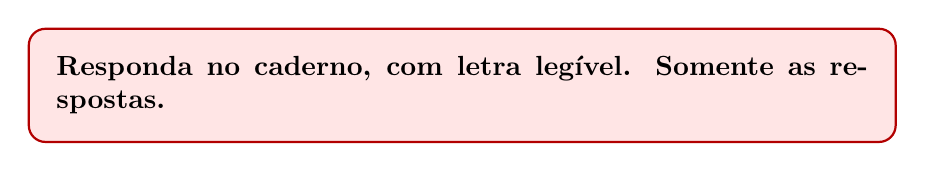
\begin{tikzpicture}
\node[rectangle, fill=red!10, rounded corners=6pt, inner sep=10pt, draw=red!70!black, thick]{
\begin{minipage}{0.85\linewidth}
\textbf{Responda no caderno, com letra legível. Somente as respostas.}
\end{minipage}
};
\end{tikzpicture}

\vspace{0.6cm}

\begin{enumerate}

\item A média aritmética é obtida somando todos os valores e dividindo pelo número de elementos. \textbf{Aplicação}: calcular a média de notas de um aluno para determinar seu desempenho final.

\item A mediana representa o valor central de um conjunto de dados quando eles estão organizados em ordem crescente.

\item A \textbf{moda} é o valor que mais se repete no conjunto; a \textbf{mediana} é o valor central. Ou seja, a moda mostra frequência e a mediana mostra posição.

\item A média pode ser puxada para cima ou para baixo quando existem valores muito altos ou muito baixos, pois todos os elementos influenciam no cálculo.

\item A mediana é mais indicada quando existem valores extremos (outliers), pois ela não é influenciada por esses valores, representando melhor o centro dos dados.

\item É importante interpretar médias porque elas permitem resumir grandes conjuntos de dados e identificar tendências gerais em tabelas e gráficos.

\item A média ponderada é calculada multiplicando cada valor por seu peso, somando os resultados e dividindo pela soma dos pesos. \textbf{Exemplo}: notas com pesos diferentes em uma avaliação.

\item Elas são importantes porque ajudam a representar um conjunto de dados de forma resumida, permitindo comparar, analisar e tirar conclusões sobre fenômenos reais.

\end{enumerate}

\end{document}

